\section{Istruzioni per l'uso}
\label{istruzioni}

Il presente capitolo offre una visione e una guida al corretto utilizzo delle principali funzionalità disponibili all'utente \textit{process owner\ped{G}}.\\
Sono presenti le seguenti sezioni:

\begin{itemize}
\item  \hyperref[autenticazione]{Autenticazione};
\item  \hyperref[home]{Navigazione nella pagina principale};
\item  \hyperref[creazione]{Creazione di un processo};
\item  \hyperref[controllo]{Controllo e approvazione di un passo};
\item  \hyperref[gestione]{Gestione di un processo};
\item  \hyperref[logout]{Chiusura della sessione}.
\end{itemize}

\pagebreak

\subsection{Autenticazione}
\label{autenticazione}

In figura \hyperref[fig:Flogin]{figura \ref{fig:Flogin}}, è rappresentata la schermata iniziale del prodotto \progetto{}, in cui viene richiesto l'inserimento dello \textit{username} e della \textit{password} dell'utente.

\begin{figure}[H] \centering 
\frame{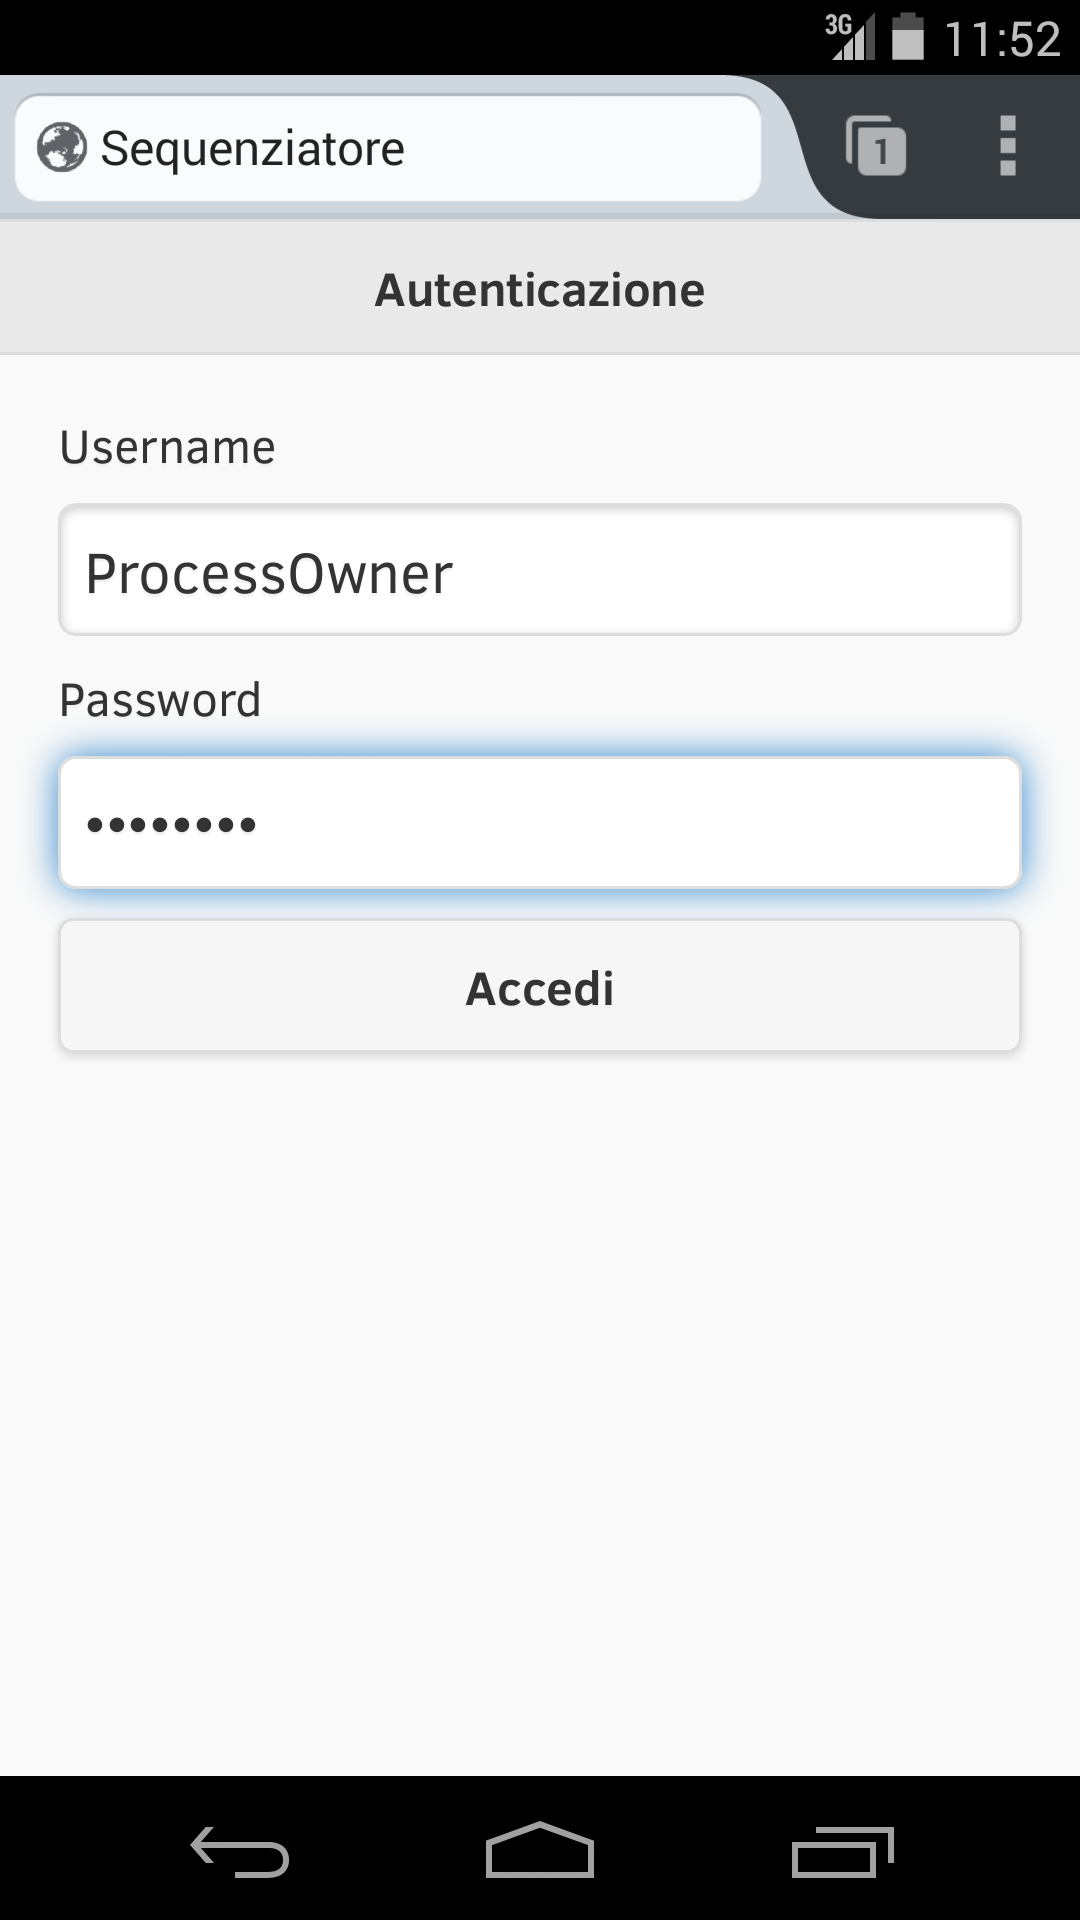
\includegraphics[width=0.5\textwidth]
{./screen/Login.png}} \caption{Schermata di autenticazione}
\label{fig:Flogin}
\end{figure}

Le credenziali di \textit{default} fornite per l'utente \textit{process owner}, sono le seguenti:
\begin{itemize}
\item \textbf{username:} ProcessOwner
\item \textbf{password:} siriusPO
\end{itemize}
Successivamente all'inserimento delle credenziali, è sufficiente selezionare il pulsante ``Accedi'', per accedere alle funzionalità dell'applicazione.

\subsubsection*{Possibili errori:}
\begin{itemize}
\item \hyperref[e1]{E1}: \textit{javascript\ped{G}} disabilitato;
\item \hyperref[e2]{E2}: credenziali non corrette;
\item \hyperref[e3]{E3}: errore di connessione al \textit{server\ped{G}}.
\end{itemize}


\subsection{Navigazione nella pagina principale}
\label{home}
In figura \hyperref[fig:Fhome]{figura \ref{fig:Fhome}}, è rappresentata la schermata della \textit{homepage} del progetto \progetto{}, accessibile dopo aver effettuato l'autenticazione, che consente di scegliere una delle funzionalità di base disponibili al \textit{process owner\ped{G}}.

\begin{figure}[H] \centering 
\frame{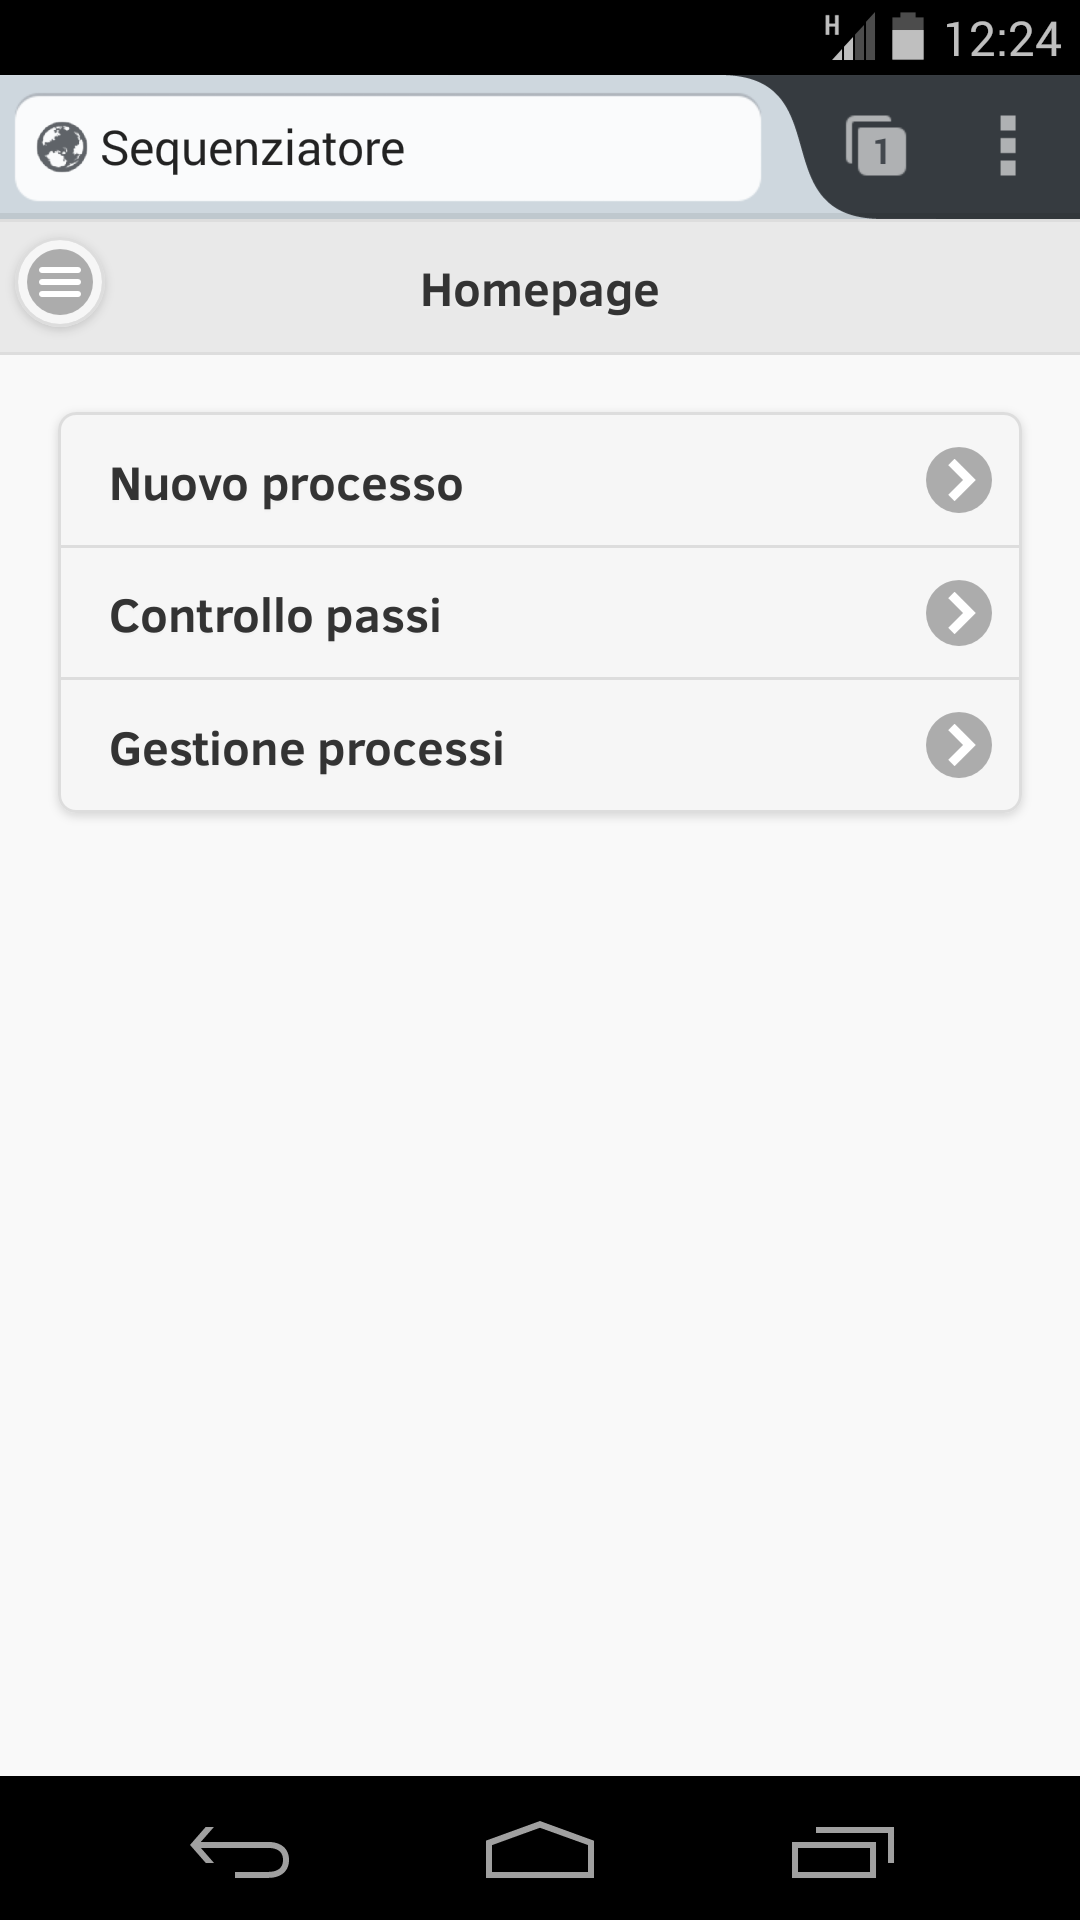
\includegraphics[width=0.5\textwidth]
{./screen/Home.png}} \caption{Homepage}
\label{fig:Fhome}
\end{figure}

È possibile selezionare uno dei seguenti pulsanti per iniziare la gestione delle rispettive funzionalità:
\begin{itemize}
\item  \hyperref[creazione]{Nuovo processo};
\item  \hyperref[controllo]{Controllo passi};
\item  \hyperref[gestione]{Gestione processi}.
\end{itemize}

Selezionando il pulsante in alto a sinistra, è possibile aprire il pannello laterale in cui è consentita la \hyperref[logout]{chiusura della sessione}.

\subsubsection*{Possibili errori:}
\begin{itemize}
\item \hyperref[e1]{E1}: \textit{javascript\ped{G}} disabilitato.
\end{itemize}

\subsection{Creazione di un processo}
\label{creazione}

\subsubsection{Definizione di un processo}
\label{definizione}
\iffalse
In figura \hyperref[fig:Fnewprocess]{figura \ref{fig:Fnewprocess}}, è rappresentata la schermata di scelta di un creazione di un processo, accessibile dopo aver effettuato l'autenticazione.

\begin{figure}[H] \centering 
\frame{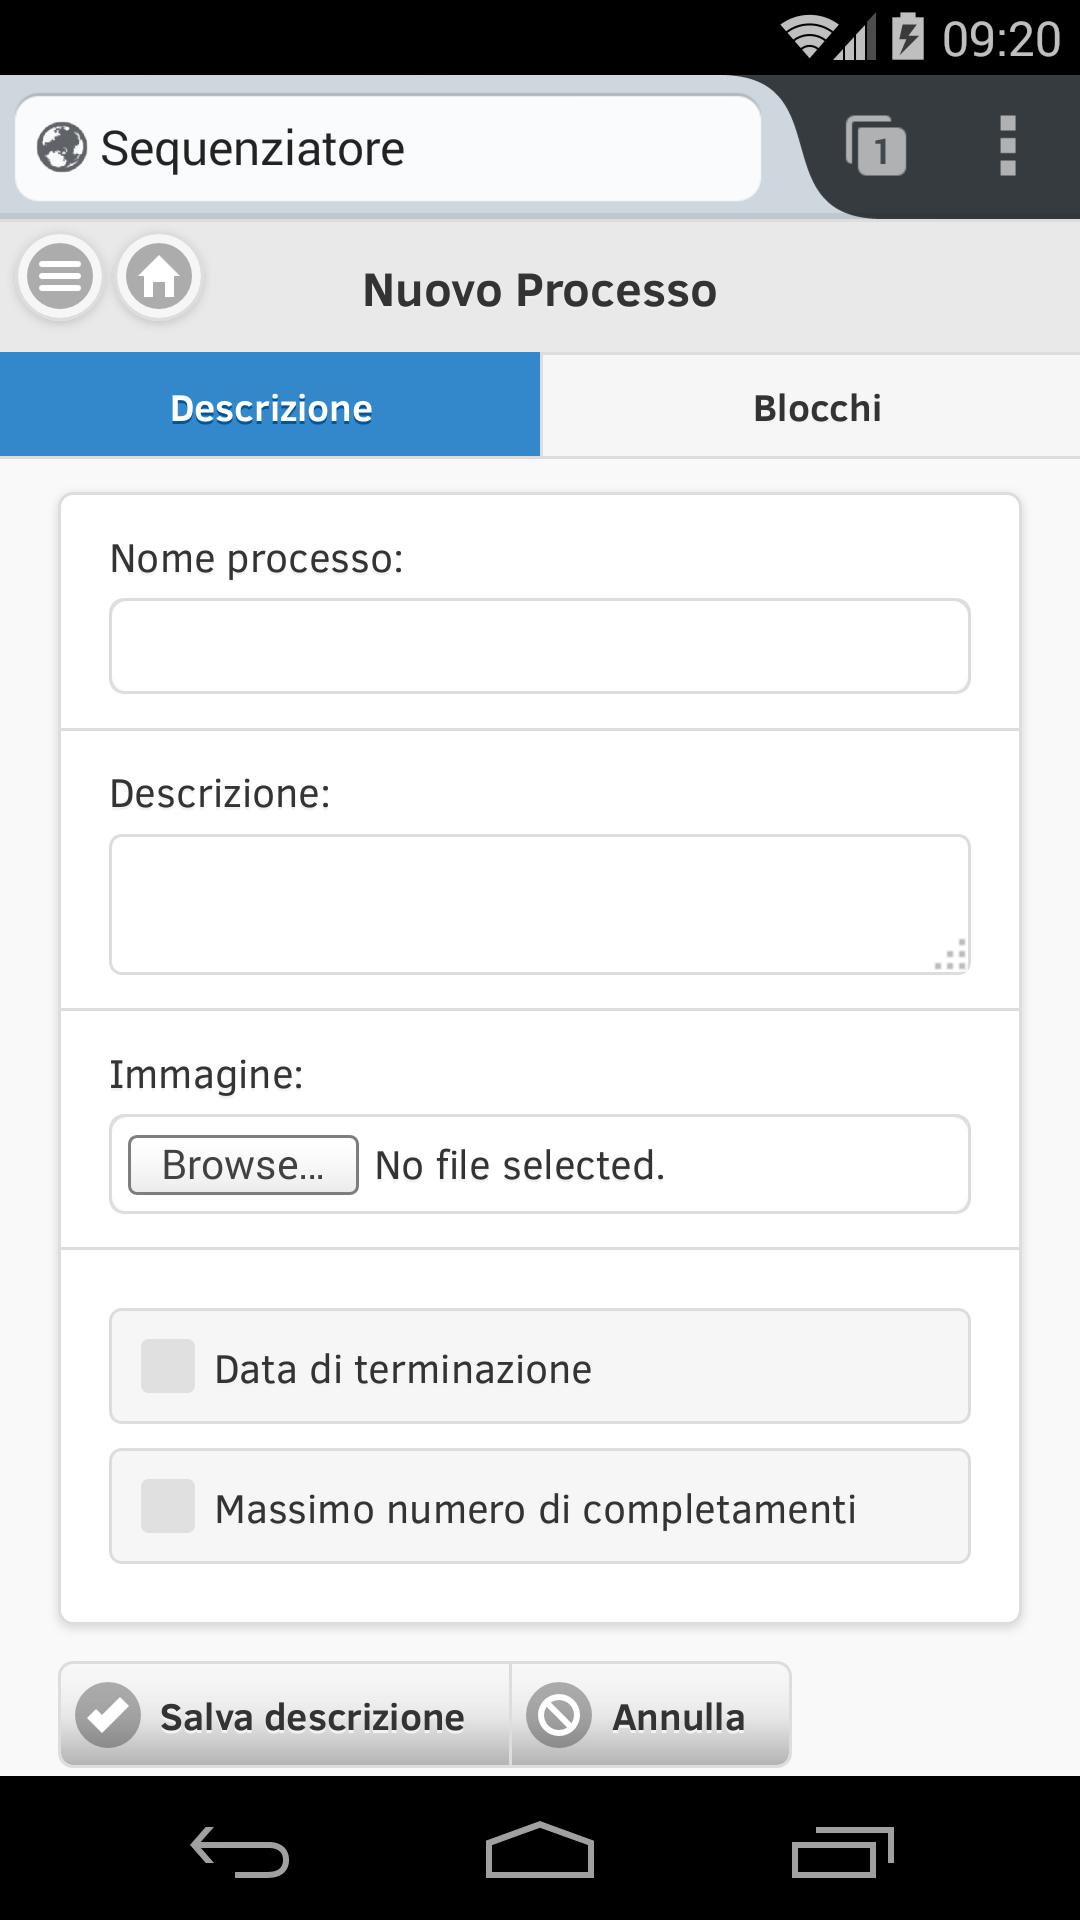
\includegraphics[width=0.5\textwidth]
{./screen/NewProcess.png}} \caption{Creazione di un processo}
\label{fig:Fcheckstep}
\end{figure}
\fi

In questa pagina è possibile definire un nuovo processo.
Viene richiesto l'inserimento dei seguenti dati:
\begin{itemize}
\item \textbf{Nome:} nome del processo, utile alla sua identificazione;
\item \textbf{Descrizione:} breve descrizione, che sarà utile agli utenti per capire lo scopo del processo;
\item \textbf{Criteri di completamento (facoltativi):} 
\begin{itemize}
\item \textbf{Data di terminazione:} Data e orario in cui il processo si concluderà in automatico;
\item \textbf{Numero massimo di completamenti:} Numero di completamenti del processo il quale, una volta raggiunto, comporta la conclusione automatica del processo.
\end{itemize}
\end{itemize}

Nella pagina sono presenti i seguenti pulsanti:
\begin{itemize}
\item \textbf{Aggiungi passo:} \hyperref[addstep]{aggiunge un passo} al processo in definizione;
\item \textbf{Salva processo:} salva il processo in definizione. Se l'operazione si conclude senza errori, il processo diventa disponibile all'iscrizione da parte degli utenti;
\item \textbf{Annulla:} ritorna alla \hyperref[home]{pagina principale}, annullando l'operazione di creazione del processo.
\end{itemize}
Per ogni passo creato sono disponibili inoltre i pulsanti:
\begin{itemize}
\item \textbf{Aggiungi criterio di superamento:} consente di aggiungere un \hyperref[vincoli]{criterio di superamento} al passo;
\item \textbf{Rimuovi passo:} rimuove il passo dal processo in definizione.
\end{itemize}
Infine in altro a sinistra sono presenti i seguenti pulsanti:
\begin{itemize}
\item \textbf{Home:} pulsante che consente di tornare alla \hyperref[home]{pagina principale};
\item \textbf{Opzioni:} apre il pannello laterale in cui è consentita la \hyperref[logout]{chiusura della sessione}.
\end{itemize}

\paragraph*{Possibili errori:}
\begin{itemize}
\item \hyperref[e1]{E1}: \textit{javascript\ped{G}} disabilitato;
\item \hyperref[e3]{E3}: errore di connessione al \textit{server\ped{G}};
\item \hyperref[e4]{E4}: nome processo già utilizzato;
\item \hyperref[e5]{E5}: dato obbligatorio mancante.
\end{itemize}

\subsubsection{Aggiunta di un passo}
\label{addstep}
\iffalse
In figura \hyperref[fig:Faddstep]{figura \ref{fig:Faddstep}}, è rappresentata la schermata di aggiunta di un passo ad un processo in definizione.

\begin{figure}[H] \centering 
\frame{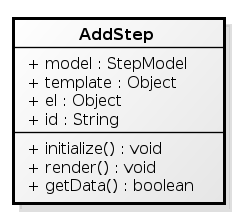
\includegraphics[width=0.5\textwidth]
{./screen/AddStep.png}} \caption{Aggiunta di un passo}
\label{fig:Faddstep}
\end{figure}
\fi

In questa pagina è possibile aggiungere un passo ad un processo in definizione.
Viene richiesto l'inserimento di una breve descrizione, che sarà utile agli utenti per capire lo scopo del passo.

Nella pagina sono presenti i seguenti pulsanti:
\begin{itemize}
\item \textbf{Aggiungi dato:} consente di aggiungere un dato al passo in definizione;
\item \textbf{Salva passo:} aggiunge il passo al processo in creazione;
\item \textbf{Annulla:} ritorna alla \hyperref[newprocess]{definizione del processo}, annullando l'operazione di aggiunta del passo.
\end{itemize}

Per ciascun passo deve essere definito un nome, utile agli utenti per capirne il significato (per esempio ``prezzo gasolio''), e deve essere selezionata una tra le seguenti tipologie:
\begin{itemize}
\item \textbf{Testuale:} gli utenti potranno inserire del testo, senza particolari vincoli;
\item \textbf{Numerico:} gli utenti potranno inserire un numero, meglio definibile da alcuni \hyperref[vincoli]{vincoli};
\item \textbf{Immagine:} gli utenti potranno inserire un'immagine caricata da \textit{file} o scattata;
\end{itemize}

Infine in altro a sinistra sono presenti i seguenti pulsanti:
\begin{itemize}
\item \textbf{Home:} pulsante che consente di tornare alla \hyperref[home]{pagina principale};
\item \textbf{Opzioni:} apre il pannello laterale in cui è consentita la \hyperref[logout]{chiusura della sessione}.
\end{itemize}

\paragraph*{Possibili errori:}
\begin{itemize}
\item \hyperref[e1]{E1}: \textit{javascript\ped{G}} disabilitato;
\item \hyperref[e5]{E5}: dato obbligatorio mancante.
\end{itemize}

\subsubsection{Aggiunta di un criterio di superamento}
\label{vincoli}
\iffalse
In figura \hyperref[fig:Fvicoli]{figura \ref{fig:Fvicoli}}, è rappresentata la schermata di aggiunta di un passo ad un processo in definizione.

\begin{figure}[H] \centering 
\frame{\includegraphics[width=0.5\textwidth]
{./screen/Vincoli.png}} \caption{Aggiunta di un criterio di superamento}
\label{fig:Fvicoli}
\end{figure}
\fi

In questa pagina è possibile aggiungere un criterio di superamento ad un passo.
Viene richiesto di inserire dei seguenti dati:
\begin{itemize}
\item \textbf{Passo successivo:} è necessario selezionare un passo, che verrà eseguito al soddisfacimento del criterio di superamento in definizione;
\item \textbf{Richiede controllo umano:} selezionare questo dato, se si vuole rendere obbligatorio il \hyperref[controllo]{controllo} da parte dell'utente \textit{process owner\ped{G}}, dei dati inviati dagli utenti che hanno soddisfatto del criterio di superamento in definizione;
\item \textbf{facoltativo:} selezionare questo dato, se si vuole rendere facoltativo il passo di cui si sta definendo un criterio di terminazione.
\end{itemize}

Per ogni dato numerico presente nel passo di cui si sta definendo un criterio di terminazione, è possibile premere il pulsante ``aggiungi vincolo'', che consente di aggiungere un vincolo numerico.
La definizione di un vincolo numerico richiede l'inserimento dei seguenti dati:
\begin{itemize}
\item \textbf{Minimo numero di cifre:} consente di stabilire il minimo numero di cifre richieste dal dato;
\item \textbf{Massimo numero di cifre:} consente di stabilire il massimo numero di cifre richieste dal dato;
\item \textbf{Valore minimo:} consente di stabilire il valore minimo assegnabile al dato;
\item \textbf{Valore massimo:} consente di stabilire il valore minimo assegnabile al dato;
\item \textbf{Numero decimale:} selezionare questo campo dati consente agli utenti di inserire cifre decimali nel dato numerico.
\end{itemize}

Nella pagina è presente il pulsante ``aggiungi vincolo geografico'' che consente di definire un vincolo sulla posizione degli utenti, necessario per soddisfare il criterio di superamento in definizione.
La definizione di un vincolo geografico richiede l'inserimento dei seguenti dati:
\begin{itemize}
\item \textbf{Latitudine} latitudine della posizione geografica richiesta dal criterio in definizione;
\item \textbf{Longitudine} longitudine della posizione geografica richiesta dal criterio in definizione;
\item \textbf{Indirizzo} (facoltativo) consente di impostare latitudine e longitudine inserendo un indirizzo;
\item \textbf{Raggio:} (facoltativo) consente di impostare un raggio in metri, entro cui, le coordinate ricevute dagli utenti, rendono il criterio di superamento in definizione soddisfatto.
\end{itemize}

Nella pagina è presente il pulsante ``aggiungi vincolo temporale'' che consente di definire un vincolo sulla data e l'ora in cui gli utenti possono inviare i dati per soddisfare il criterio di superamento in definizione.
La definizione di un vincolo temporale richiede l'inserimento di almeno uno dei seguenti dati:
\begin{itemize}
\item \textbf{inizio} data e ora da cui è possibile inviare i dati per soddisfare il criterio di superamento in definizione;
\item \textbf{fine} data e ora entro cui è obbligatorio inviare i dati per soddisfare il criterio di superamento in definizione.
\end{itemize}

Ogni vincolo può essere salvato premendo il pulsante ``Salva vincolo'', o può esserne annullata la creazione prendo il pulsante ``Annulla''.

Nella pagina sono presenti i seguenti pulsanti:
\begin{itemize}
\item \textbf{Salva criterio:} consente di salvare il criterio di superamento in definizione;
\item \textbf{Annulla:} ritorna alla \hyperref[newprocess]{definizione del processo}, annullando l'operazione di definizione del criterio di superamento.
\end{itemize}

Infine in altro a sinistra sono presenti i seguenti pulsanti:
\begin{itemize}
\item \textbf{Home:} pulsante che consente di tornare alla \hyperref[home]{pagina principale};
\item \textbf{Opzioni:} apre il pannello laterale in cui è consentita la \hyperref[logout]{chiusura della sessione}.
\end{itemize}

\paragraph*{Possibili errori:}
\begin{itemize}
\item \hyperref[e1]{E1}: \textit{javascript\ped{G}} disabilitato;
\item \hyperref[e5]{E5}: dato obbligatorio mancante.
\end{itemize}

\subsection{Controllo e approvazione di un passo}
\label{controllo}

\subsubsection{Scelta di un passo in attesa di approvazione}

In figura \hyperref[fig:Fcheckstep]{figura \ref{fig:Fcheckstep}}, è rappresentata la schermata di scelta di un passo che richiede intervento umano, accessibile dopo aver effettuato l'autenticazione.

\begin{figure}[H] \centering 
\frame{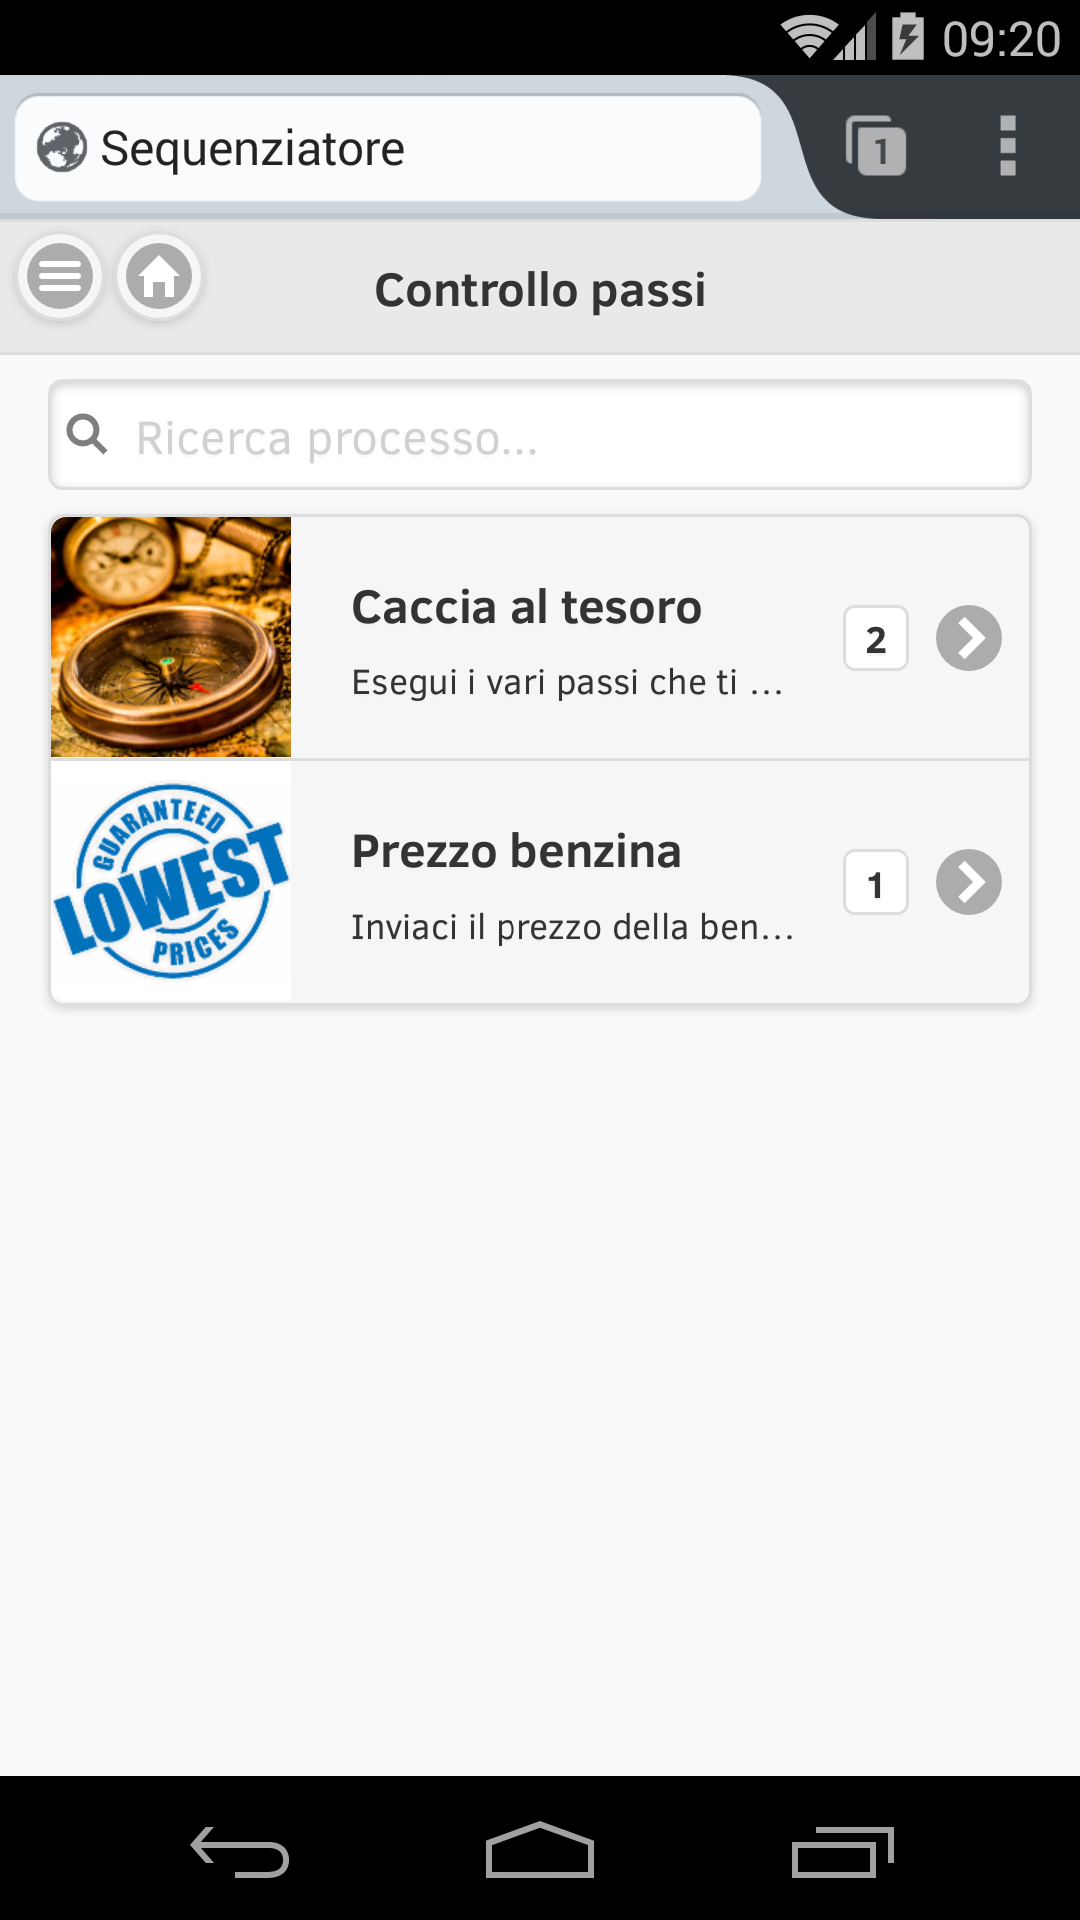
\includegraphics[width=0.5\textwidth]
{./screen/CheckStep.png}} \caption{Scelta di un passo che richiede approvazione}
\label{fig:Fcheckstep}
\end{figure}

In questa pagina è possibile selezionare uno tra i passi in elenco. È inoltre disponibile la funzionalità di ricerca: inserendo del testo nella barra di ricerca, l'elenco si aggiornerà, con i soli passi che contengono nella descrizione o nell'username dell'utente che ha inviato i dati, il testo oggetto della ricerca.
Per ripristinare l'elenco è sufficiente cancellare il testo nella barra dell'elenco.

In altro a sinistra sono presenti i seguenti pulsanti:
\begin{itemize}
\item \textbf{Home:} pulsante che consente di tornare alla \hyperref[home]{pagina principale};
\item \textbf{Opzioni:} apre il pannello laterale in cui è consentita la \hyperref[logout]{chiusura della sessione}.
\end{itemize}

\paragraph*{Possibili errori:}
\begin{itemize}
\item \hyperref[e1]{E1}: \textit{javascript\ped{G}} disabilitato;
\item \hyperref[e3]{E3}: errore di connessione al \textit{server\ped{G}}.
\end{itemize}

\subsubsection{Approvazione di un passo}

In figura \hyperref[fig:Fapprove]{figura \ref{fig:Fapprove}}, è rappresentata la schermata di visualizzazione dei dati di un passo che richiede approvazione, accessibile dopo aver effettuato l'autenticazione.

\begin{figure}[H] \centering 
\frame{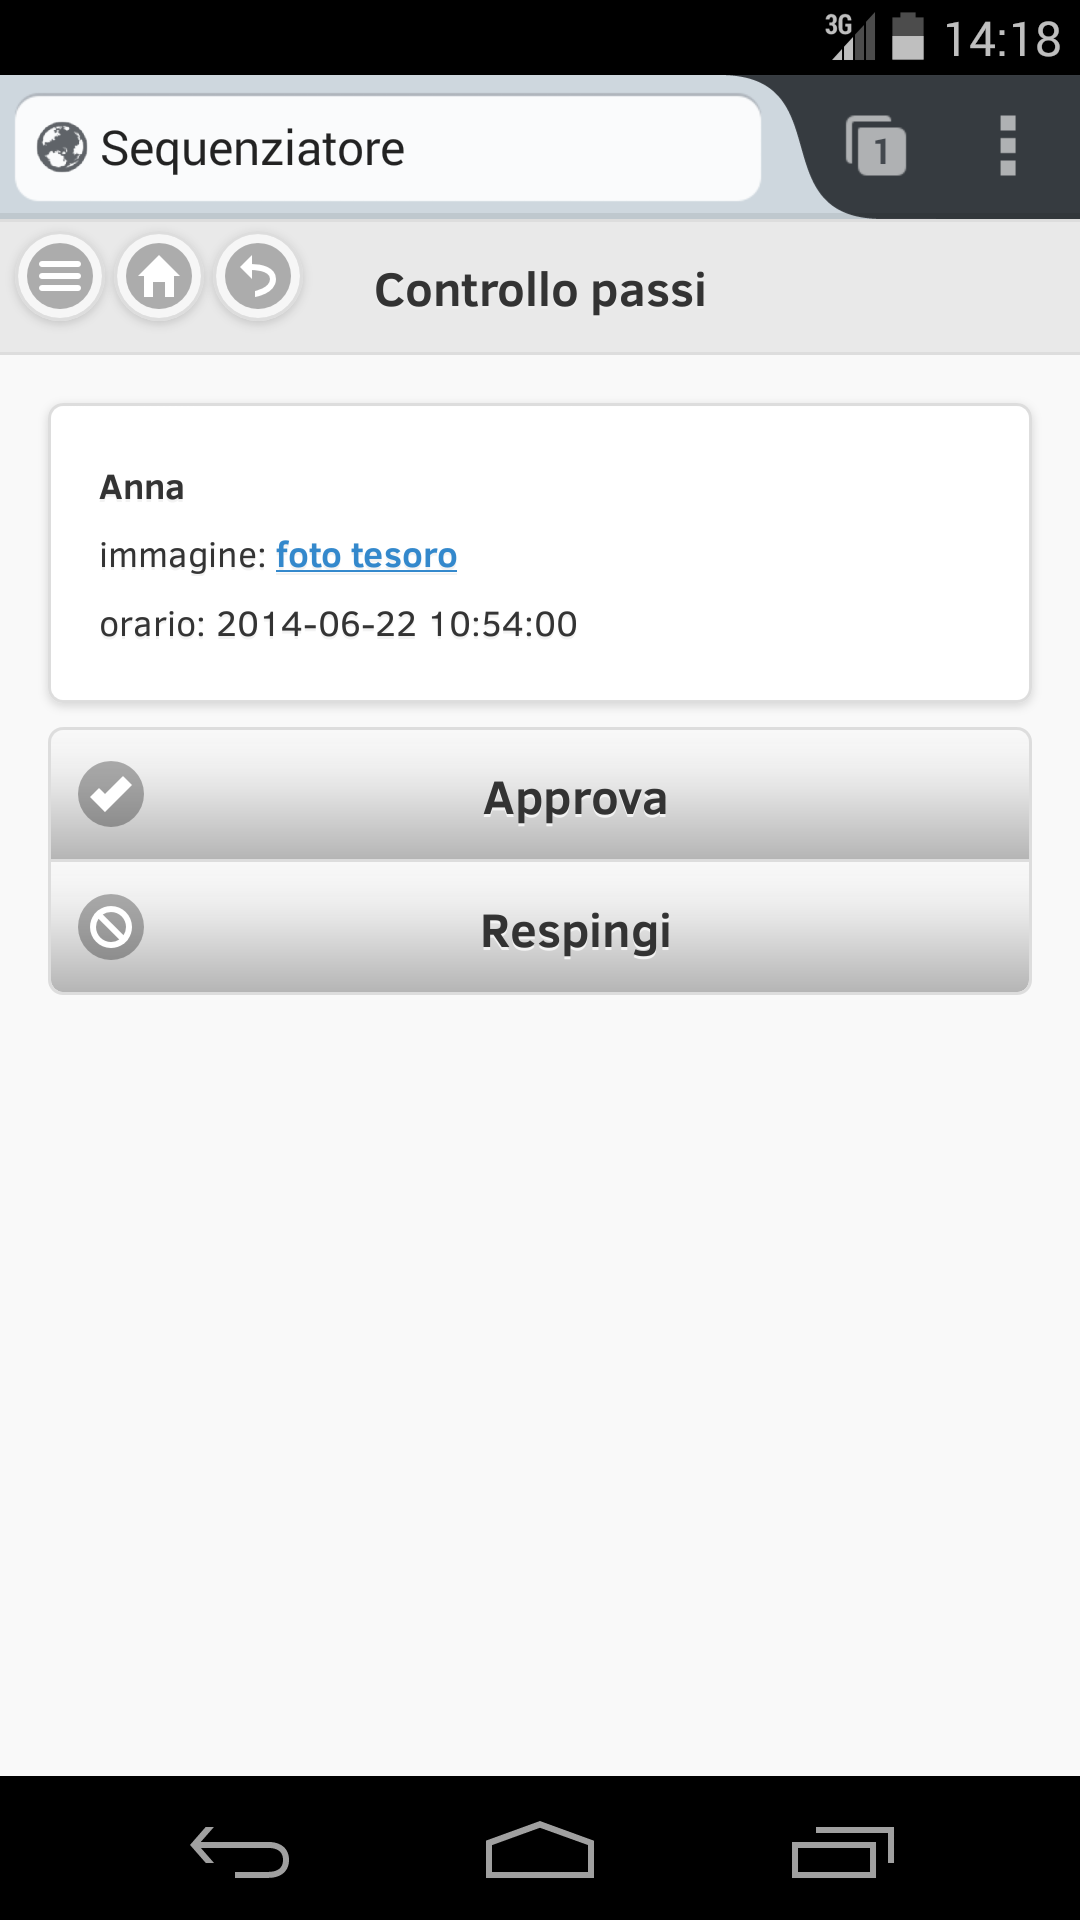
\includegraphics[width=0.5\textwidth]
{./screen/Approve.png}} \caption{Visualizzazione dei dati di un passo}
\label{fig:Fapprove}
\end{figure}

Questa pagina contiene l'elenco dei dati da un utente riguardanti il passo selezionato. 
Premendo il pulsante ``Approva'' è possibile approvare il passo selezionato, mentre, premendo il pulsante ``respingi'' il passo verrà respinto. In entrami i casi, l'esito viene inviato all'utente interessato.

In altro a sinistra sono presenti i seguenti pulsanti:
\begin{itemize}
\item \textbf{Home:} pulsante che consente di tornare alla \hyperref[home]{pagina principale};
\item \textbf{Opzioni:} apre il pannello laterale in cui è consentita la \hyperref[logout]{chiusura della sessione};
\item \textbf{Indietro:} pulsante che consente di tornare alla scelta di un passo in attesa di approvazione.
\end{itemize}

\paragraph*{Possibili errori:}
\begin{itemize}
\item \hyperref[e1]{E1}: \textit{javascript\ped{G}} disabilitato;
\item \hyperref[e3]{E3}: errore di connessione al \textit{server\ped{G}}.
\end{itemize}


\subsection{Gestione di un processo}
\label{gestione}

\subsubsection{Scelta di un processo}

In figura \hyperref[fig:Fprocesses]{figura \ref{fig:Fprocesses}}, è rappresentata la schermata di gestione dei processi, accessibile dopo aver effettuato l'autenticazione, che consente di selezionare un processo per gestirlo.

\begin{figure}[H] \centering 
\frame{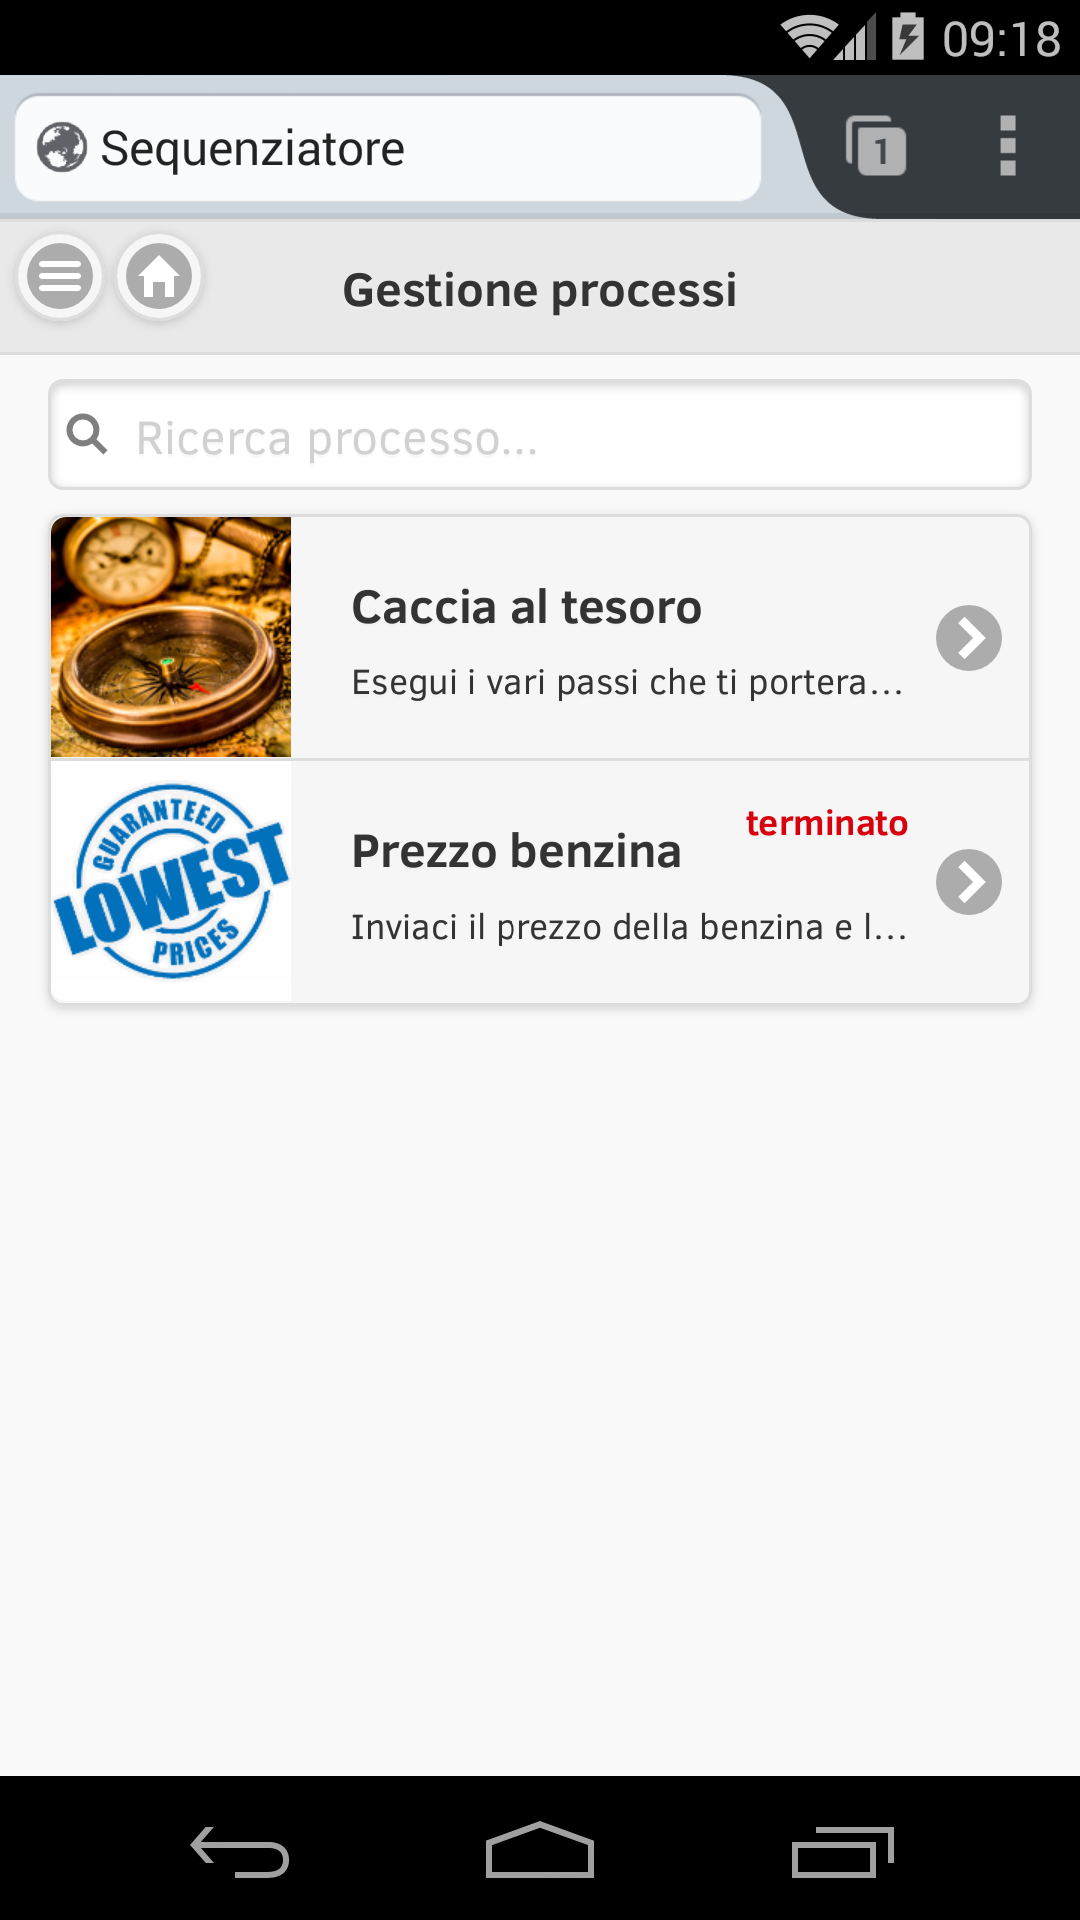
\includegraphics[width=0.5\textwidth]
{./screen/Processes.png}} \caption{Scelta processo}
\label{fig:Fprocesses}
\end{figure}

In questa pagina è possibile selezionare uno tra i processi in elenco. È inoltre disponibile la funzionalità di ricerca: inserendo del testo nella barra di ricerca (con suscritto ``Ricerca processo''), l'elenco si aggiornerà, con i soli processi che contengono nel titolo o nella descrizione, il testo oggetto della ricerca.
Per ripristinare l'elenco è sufficiente cancellare il testo nella barra dell'elenco, o premere il pulsante a forma di ``x''.

In altro a sinistra sono presenti i seguenti pulsanti:
\begin{itemize}
\item \textbf{Home:} pulsante che consente di tornare alla \hyperref[home]{pagina principale};
\item \textbf{Opzioni:} apre il pannello laterale in cui è consentita la \hyperref[logout]{chiusura della sessione}.
\end{itemize}

\paragraph*{Possibili errori:}
\begin{itemize}
\item \hyperref[e1]{E1}: \textit{javascript\ped{G}} disabilitato;
\item \hyperref[e3]{E3}: errore di connessione al \textit{server\ped{G}}.
\end{itemize}

\subsubsection{Scelta di un passo del processo}

In figura \hyperref[fig:Fprocess]{figura \ref{fig:Fprocess}}, è rappresentata la schermata di gestione di un processo, accessibile dopo aver effettuato l'autenticazione, che consente di selezionare un passo del processo in gestione.

\begin{figure}[H] \centering 
\frame{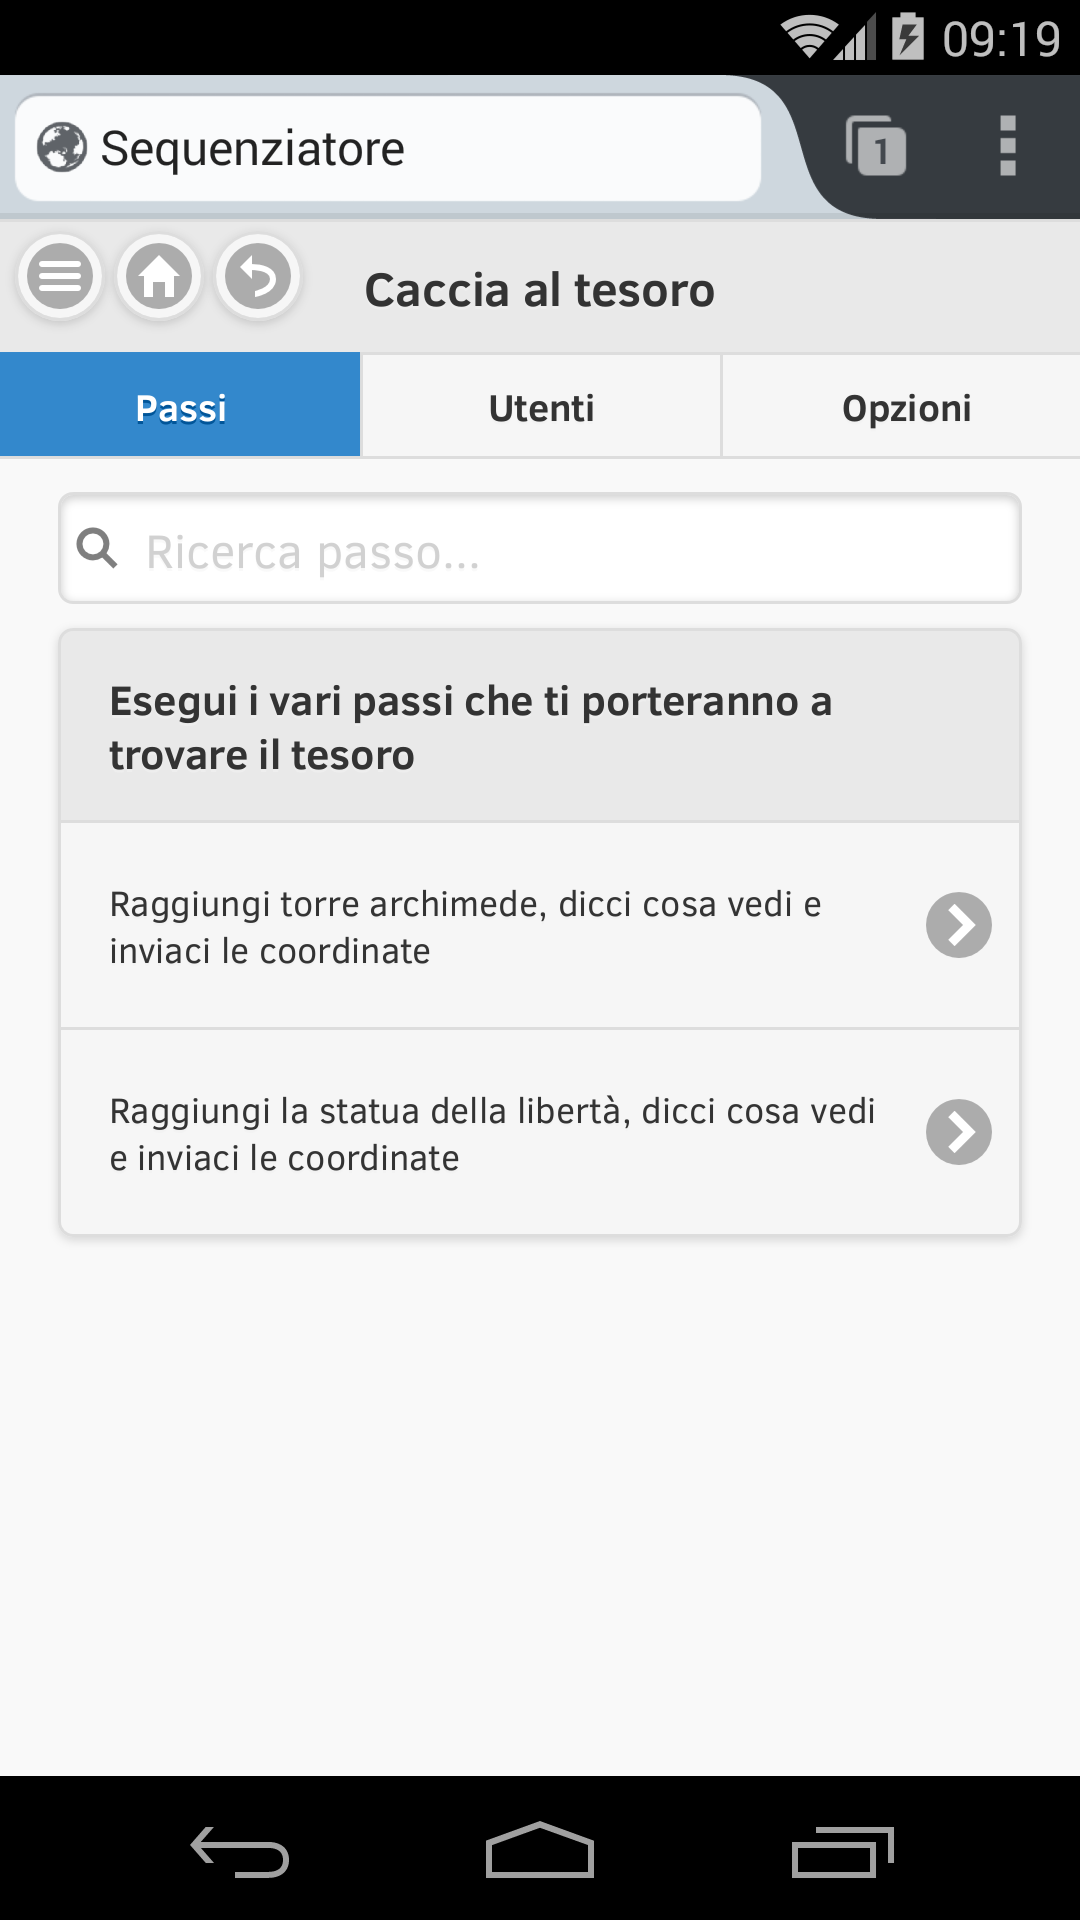
\includegraphics[width=0.5\textwidth]
{./screen/Process.png}} \caption{Scelta di un passo}
\label{fig:Fprocess}
\end{figure}

In questa pagina è possibile selezionare uno tra i passi in elenco. È inoltre disponibile la funzionalità di ricerca: inserendo del testo nella barra di ricerca, l'elenco si aggiornerà, con i soli passi che contengono nella descrizione, il testo oggetto della ricerca.
Per ripristinare l'elenco è sufficiente cancellare il testo nella barra dell'elenco.

In altro a sinistra sono presenti i seguenti pulsanti:
\begin{itemize}
\item \textbf{Home:} pulsante che consente di tornare alla \hyperref[home]{pagina principale};
\item \textbf{Opzioni:} apre il pannello laterale in cui è consentita la \hyperref[logout]{chiusura della sessione};
\item \textbf{Indietro:} pulsante che consente di tornare alla scelta di un processo.
\end{itemize}

\paragraph*{Possibili errori:}
\begin{itemize}
\item \hyperref[e1]{E1}: \textit{javascript\ped{G}} disabilitato;
\item \hyperref[e3]{E3}: errore di connessione al \textit{server\ped{G}}.
\end{itemize}

\subsubsection{Visualizzazione dei dati di un passo}

In figura \hyperref[fig:Fstepdata]{figura \ref{fig:Fstepdata}}, è rappresentata la schermata di visualizzazione dei dati di un passo, accessibile dopo aver effettuato l'autenticazione.

\begin{figure}[H] \centering 
\frame{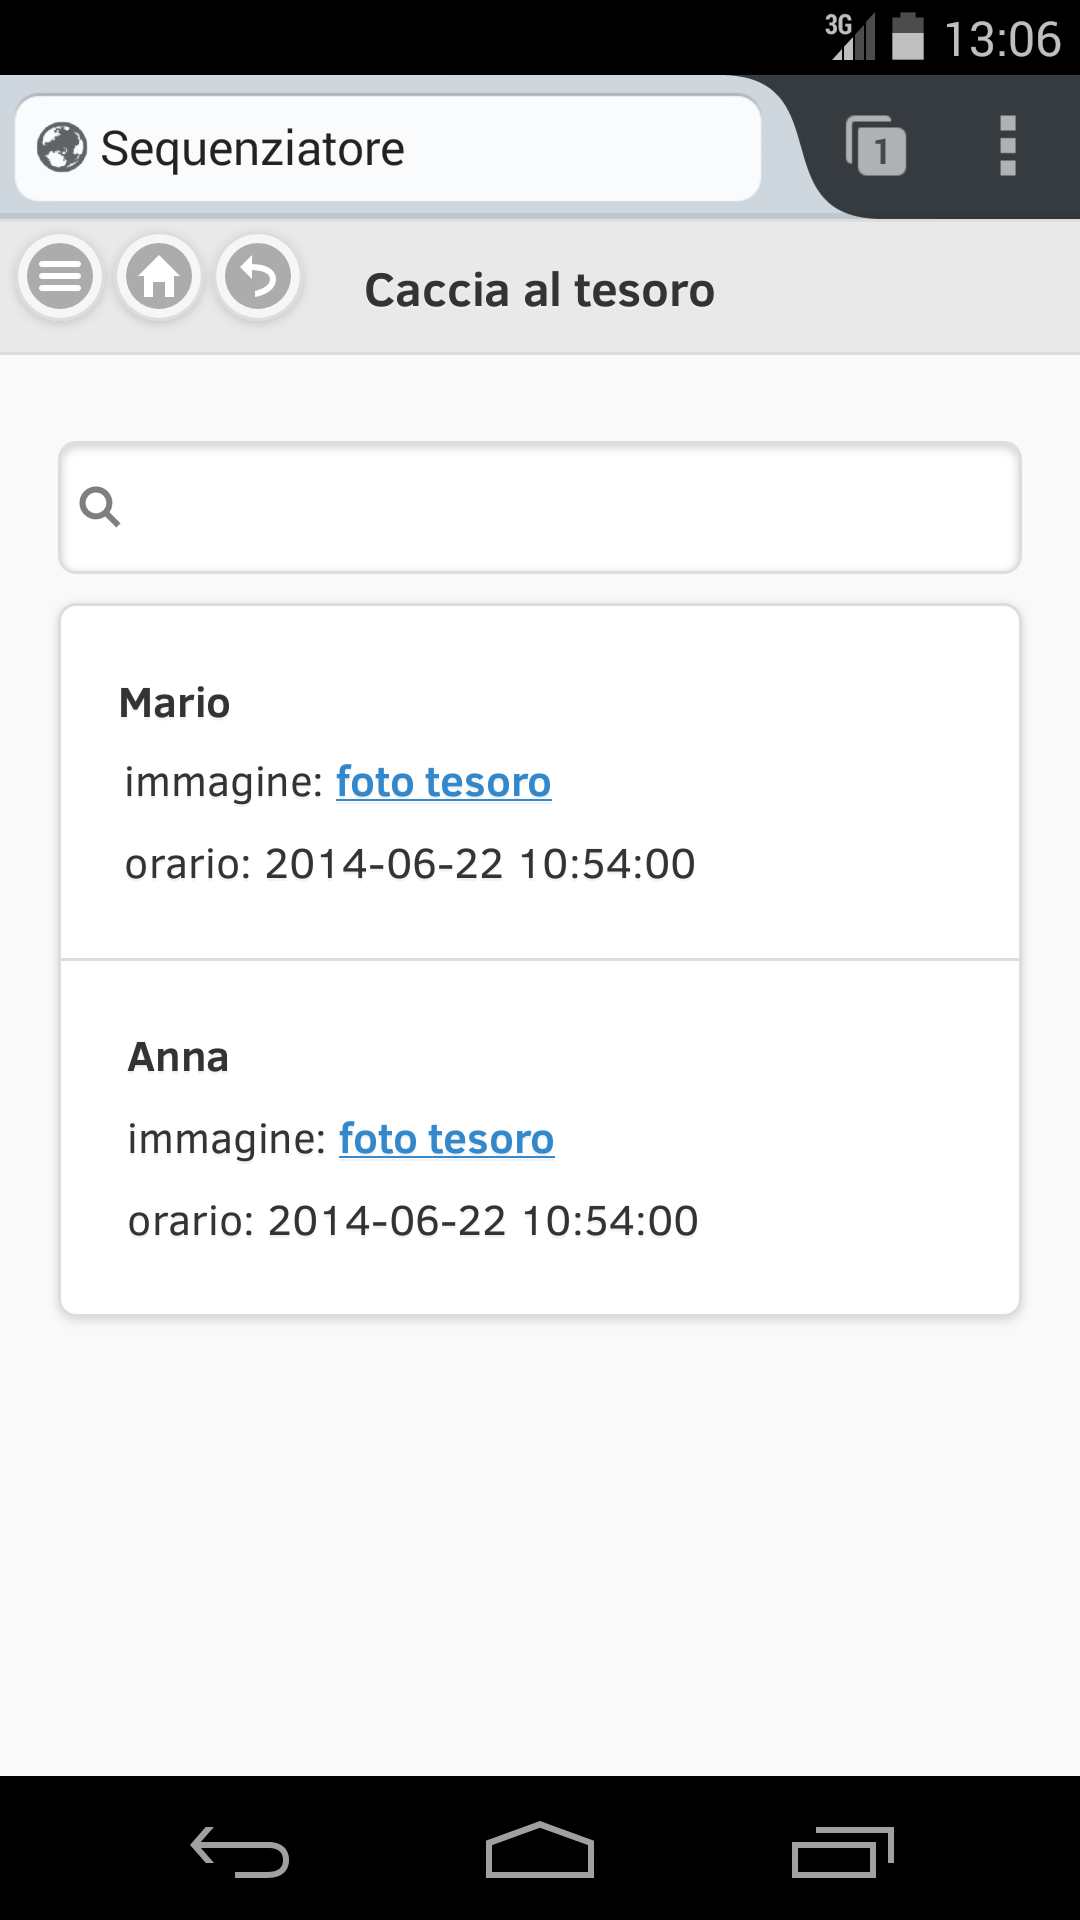
\includegraphics[width=0.5\textwidth]
{./screen/StepData.png}} \caption{Visualizzazione dei dati di un passo}
\label{fig:Fstepdata}
\end{figure}

Questa pagina è composta dall'elenco dei dati inviati dagli utenti riguardanti il passo selezionato. 
È disponibile la funzionalità di ricerca: inserendo del testo nella barra di ricerca, l'elenco si aggiornerà, con i soli dati che contengono nella descrizione, il testo oggetto della ricerca.
Per ripristinare l'elenco è sufficiente cancellare il testo nella barra dell'elenco.

In altro a sinistra sono presenti i seguenti pulsanti:
\begin{itemize}
\item \textbf{Home:} pulsante che consente di tornare alla \hyperref[home]{pagina principale};
\item \textbf{Opzioni:} apre il pannello laterale in cui è consentita la \hyperref[logout]{chiusura della sessione};
\item \textbf{Indietro:} pulsante che consente di tornare alla scelta di un passo del processo in gestione.
\end{itemize}

\paragraph*{Possibili errori:}
\begin{itemize}
\item \hyperref[e1]{E1}: \textit{javascript\ped{G}} disabilitato;
\item \hyperref[e3]{E3}: errore di connessione al \textit{server\ped{G}}.
\end{itemize}

\subsection{Chiusura della sessione}
\label{logout}
In figura \hyperref[fig:Flogout]{figura \ref{fig:Flogout}}, è rappresentato il pannello laterale, visualizzabile premendo il pulsante opzioni (vedi pulsante in alto a sinistra in \hyperref[fig:Fhome]{figura \ref{fig:Fhome}}), da qualsiasi pagina accessibile dopo aver effettuato l'autenticazione.

\begin{figure}[H] \centering 
\frame{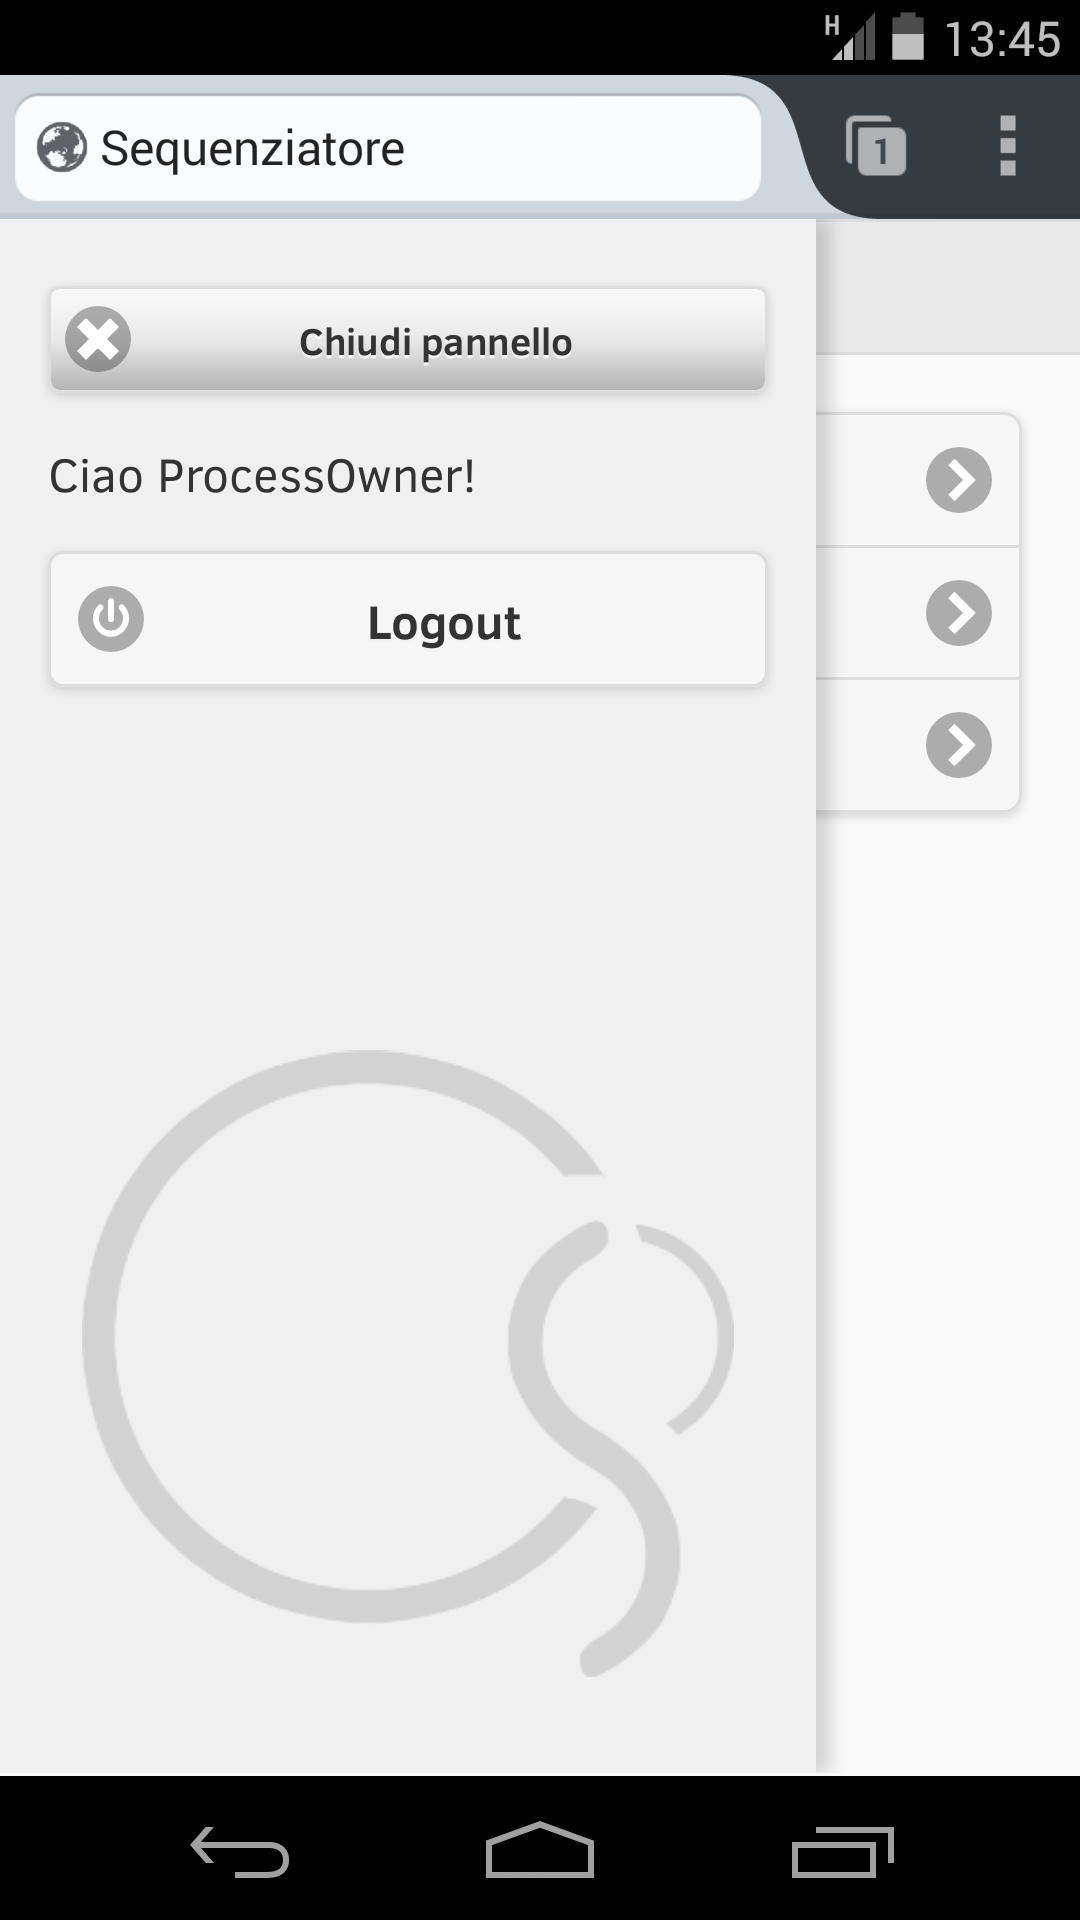
\includegraphics[width=0.5\textwidth]
{./screen/Logout.png}} \caption{Pannello laterale}
\label{fig:Flogout}
\end{figure}

Premendo il pulsante ``chiudi pannello'' è possibile ritornare alla pagina da cui il pannello è stato aperto.
Premendo il pulsante ``Logout'' l'utente ritornerà alla pagina di \hyperref[autenticazione]{autenticazione}, e i suoi dati di sessione\ped{G} vengono eliminati.

\subsubsection*{Possibili errori:}
\begin{itemize}
\item \hyperref[e1]{E1}: \textit{javascript\ped{G}} disabilitato.
\end{itemize}